\documentclass[a4paper, czech]{article}

\title{
	\begin{framed}
		\setstretch{1.5}
		{\large Audio elektronika (BPC/BKC-AUD)}\\
		Laboratorní úloha č. 7 (protokol)\\
		\textbf{Digitální vícepásmový ekvalizer a limiter}
	\end{framed}
	}
\author{Karolína A. Šebestová}
\date{7. 4. 2026, 11:00}

\usepackage[czech]{babel}
\usepackage{indentfirst}
\usepackage{graphicx}
\usepackage{float}
\usepackage[margin=1.5cm]{geometry}
\usepackage{booktabs}
\usepackage{amsmath}
\usepackage{multirow}
\usepackage{colortbl}
\usepackage{framed} % \begin{framed}
\usepackage{setspace} % \setstretch{}
\usepackage{siunitx}
\usepackage{xcolor}

\sisetup{locale = DE}

\begin{document}

\maketitle

\section{Měření}

\subsection{Měření modulových kmitočtových charakteristik}

\begin{table}[H]
    \centering
    \catcode`\-=12
    \caption{Zvolené parametry ekvalizeru levého kanálu.}

    \begin{tabular}{cccccccc}
        \toprule
        \textbf{$f$ [Hz]} & 60 & 180 & 430 & 1\,000 & 3\,000 & 7\,300 & 15\,000 \\
        \cmidrule(rl){1-8}
        \textbf{$A_u$ [dB]} & 0 & 0 & 5 & 5 & 5 & 0 & 0 \\
        \bottomrule
    \end{tabular}
\end{table}

\begin{table}[H]
    \centering
    \catcode`\-=12
    \caption{Modulové kmitočtové charakteristiky pro různá nastavení ekvalizeru.}
    \begin{tabular}{ccccccccc}
        \toprule
        \textbf{stopa} & \textbf{$f$ [Hz]} & \textbf{$U_1$ [mV]} & \textbf{$U_{21}$ [mV]} & \textbf{$A_1$ [dB]} & \textbf{$U_{22}$ [mV]} & \textbf{$A_2$ [dB]} & \textbf{$U_{23}$ [mV]} & \textbf{$A_3$ [dB]} \\
        \cmidrule(rl){1-2}
        \cmidrule(rl){3-3}
        \cmidrule(rl){4-5}
        \cmidrule(rl){6-7}
        \cmidrule(rl){8-9}
        7     & 20     & 962     & 853      & -1,04   & 747      & -2,20   & 749      & -2,17   \\
        9     & 31,5   & 954     & 1041     & 0,76    & 761      & -1,96   & 765      & -1,92   \\
        11    & 50     & 968     & 1390     & 3,14    & 791      & -1,75   & 797      & -1,69   \\
        13    & 80     & 970     & 1410     & 3,25    & 805      & -1,62   & 818      & -1,48   \\
        15    & 125    & 957     & 1410     & 3,37    & 806      & -1,49   & 839      & -1,14   \\
        17    & 200    & 969     & 1630     & 4,52    & 811      & -1,55   & 916      & -0,49   \\
        19    & 315    & 957     & 1370     & 3,12    & 816      & -1,38   & 1201     & 1,97    \\
        21    & 500    & 968     & 1370     & 3,02    & 821      & -1,43   & 1470     & 3,63    \\
        23    & 800    & 969     & 940      & -0,26   & 841      & -1,23   & 1480     & 3,68    \\
        25    & 1\,250   & 957     & 841      & -1,12   & 918      & -0,36   & 1370     & 3,12    \\
        27    & 2\,000   & 969     & 822      & -1,43   & 1161     & 1,57    & 1268     & 2,34    \\
        29    & 3\,150   & 958     & 800      & -1,57   & 1500     & 3,89    & 1460     & 3,66    \\
        31    & 5\,000   & 969     & 803      & -1,63   & 1310     & 2,62    & 1033     & 0,56    \\
        33    & 8\,000   & 966     & 798      & -1,66   & 1470     & 3,65    & 863      & -0,98   \\
        35    & 12\,500  & 944     & 782      & -1,64   & 1169     & 1,86    & 802      & -1,42   \\
        37    & 20\,000  & 923     & 752      & -1,78   & 783      & -1,43   & 756      & -1,73  \\
        \bottomrule
    \end{tabular}
\end{table}

\begin{figure}[H]
    \centering
    
\includegraphics[width=\textwidth]{grafy/graf1.pdf}
    \caption{Modulová kmitočtová charakteristika při zdůraznění hloubek ekvalizeru.}
\end{figure}

\begin{figure}[H]
    \centering
    
\includegraphics[width=\textwidth]{grafy/graf2.pdf}
    \caption{Modulová kmitočtová charakteristika při zdůraznění výšek ekvalizeru.}
\end{figure}

\begin{figure}[H]
    \centering
    
\includegraphics[width=\textwidth]{grafy/graf3.pdf}
    \caption{Modulová kmitočtová charakteristika při vlastním nastavení ekvalizeru.}
\end{figure}

\subsection{Měření převodních charakteristik pro různé nastavení křivky limiteru}

\begin{table}[H]
    \centering
    \catcode`\-=12
    \caption{Převodní charakteristika limiteru.}
    \begin{tabular}{ccccc}
        \toprule
        \textbf{stopa} & \textbf{$U_1$ [mV]} & \textbf{$U_{21}$ [mV]} & \textbf{$U_{22}$ [mV]} & \textbf{$U_{23}$ [mV]} \\
        \cmidrule(rl){1-5}
        15    & 1790    & 1480     & 599      & 281      \\
        16    & 1430    & 1184     & 569      & 290      \\
        17    & 1008    & 841      & 465      & 290      \\
        18    & 637     & 543      & 384      & 280      \\
        19    & 201     & 198      & 196      & 197      \\
        \bottomrule
    \end{tabular}
\end{table}

\begin{figure}[H]
    \centering
    
\includegraphics[width=\textwidth]{grafy/graf4.pdf}
    \caption{Převodní charakteristika pro vypnutý limiter.}
\end{figure}

\begin{figure}[H]
    \centering
    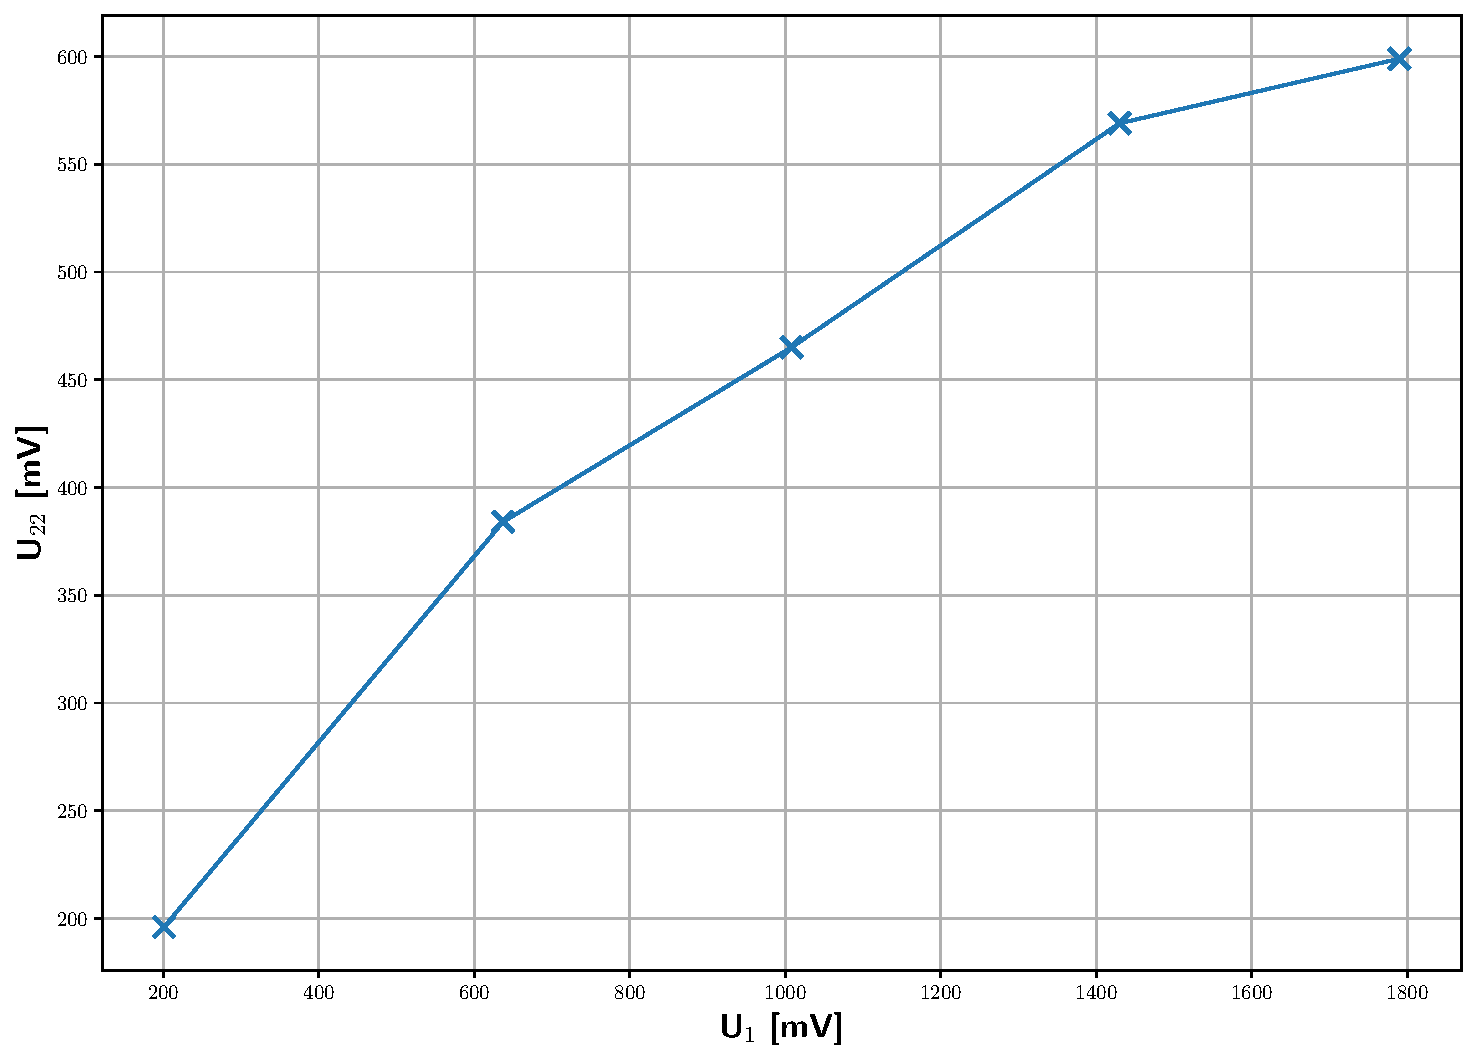
\includegraphics[width=\textwidth]{grafy/graf5.pdf}
    \caption{Převodní charakteristika pro přednastavenou kompresní křivku „compress2“.}
\end{figure}

\begin{figure}[H]
    \centering
    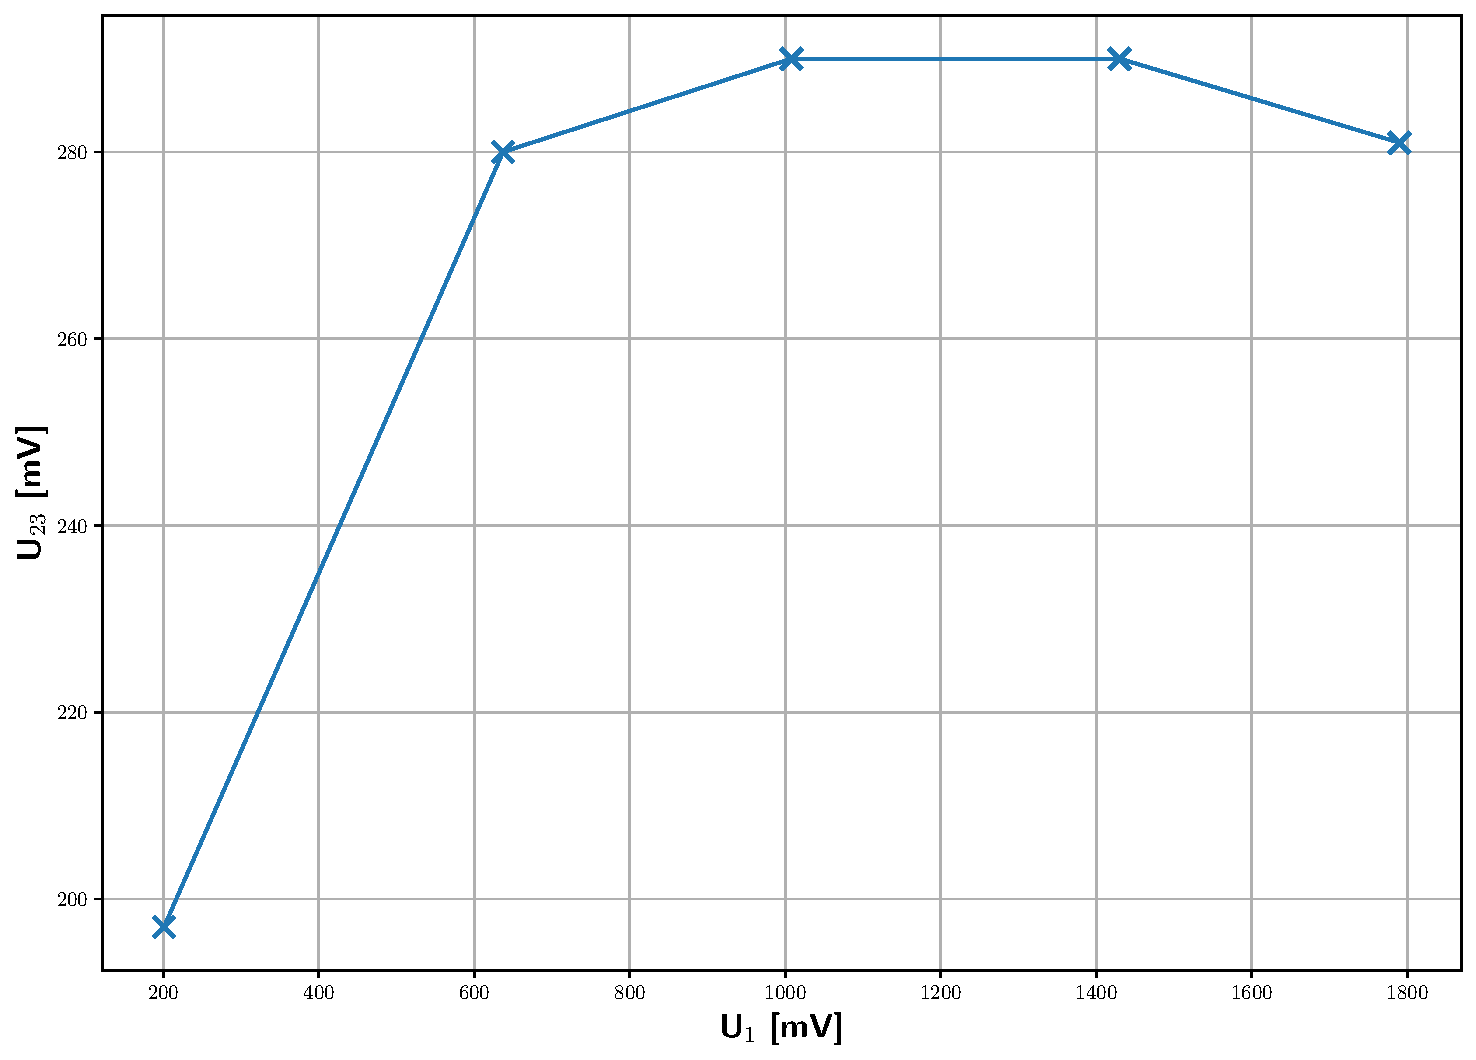
\includegraphics[width=\textwidth]{grafy/graf6.pdf}
    \caption{Převodní charakteristika pro vlastní nastavení – limitaci.}
\end{figure}

\subsection{Automatické měření kmitočtové charakteristiky}

\begin{figure}[H]
    \centering
    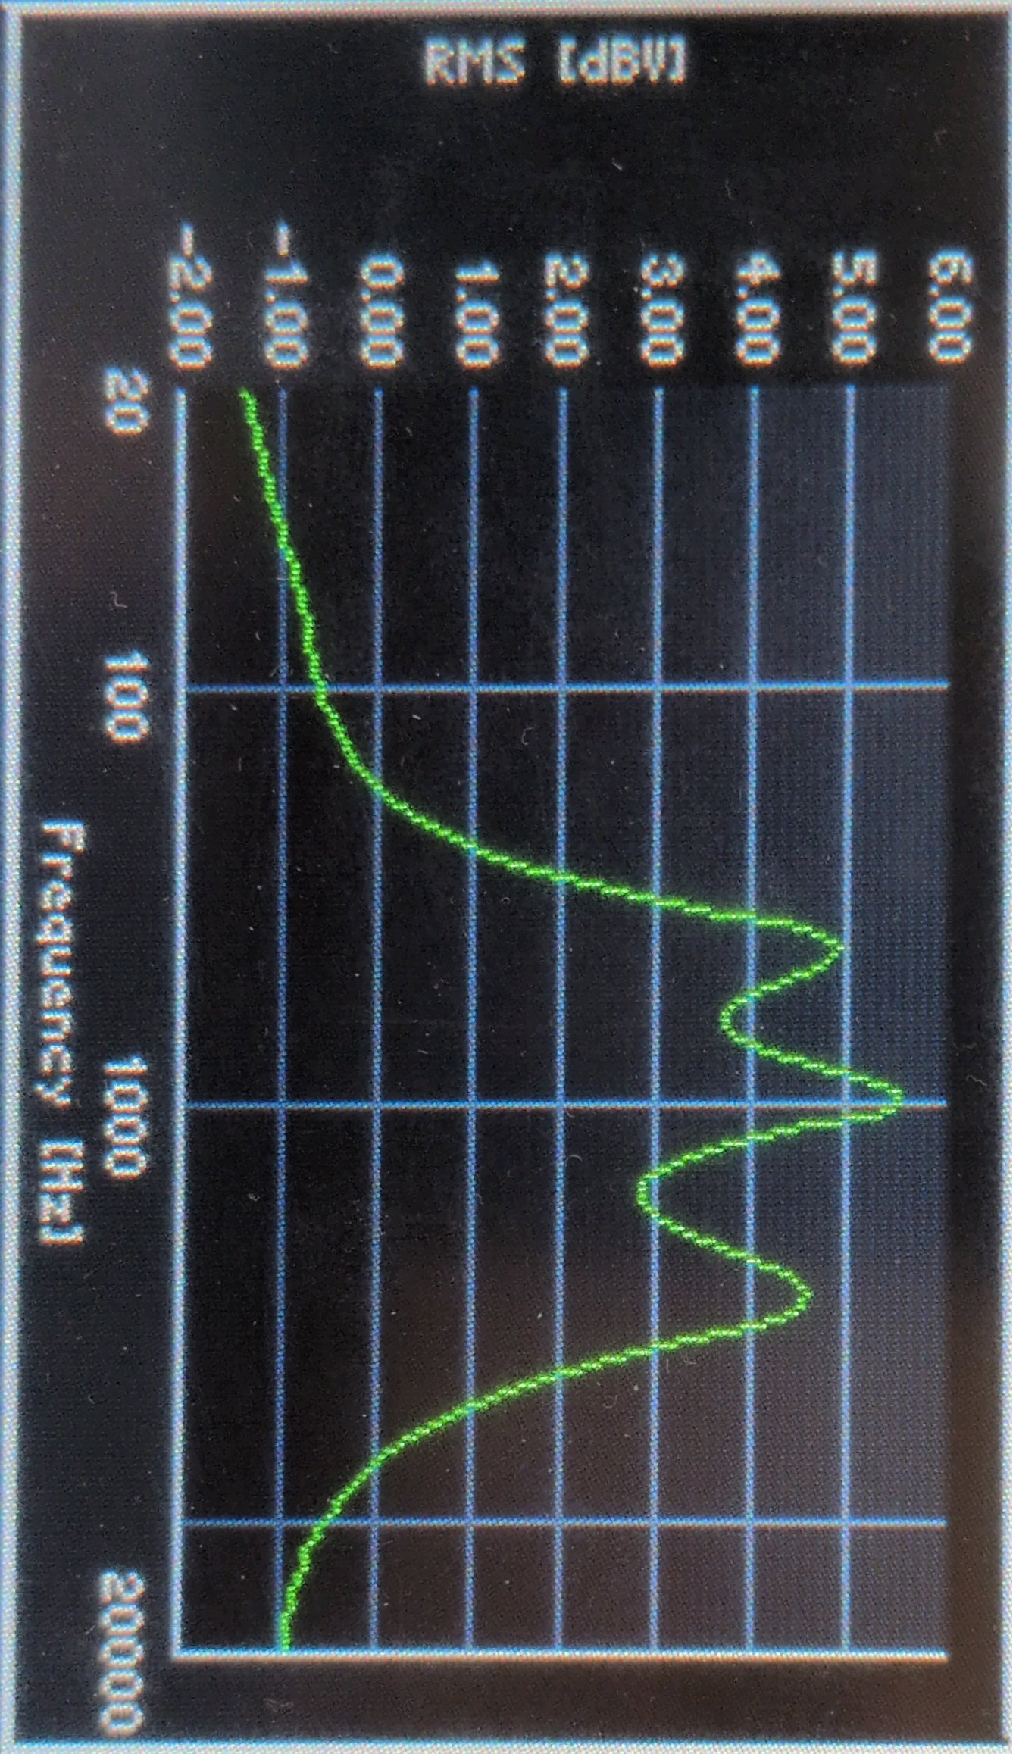
\includegraphics[height=\textwidth, angle=90]{osciloskop/5_automaticka_kmit_char.pdf}
    \caption{Automatické měření kmitočtové charakteristiky.}
\end{figure}

\subsection{Kontrola fáze}

\begin{figure}[H]
    \centering
    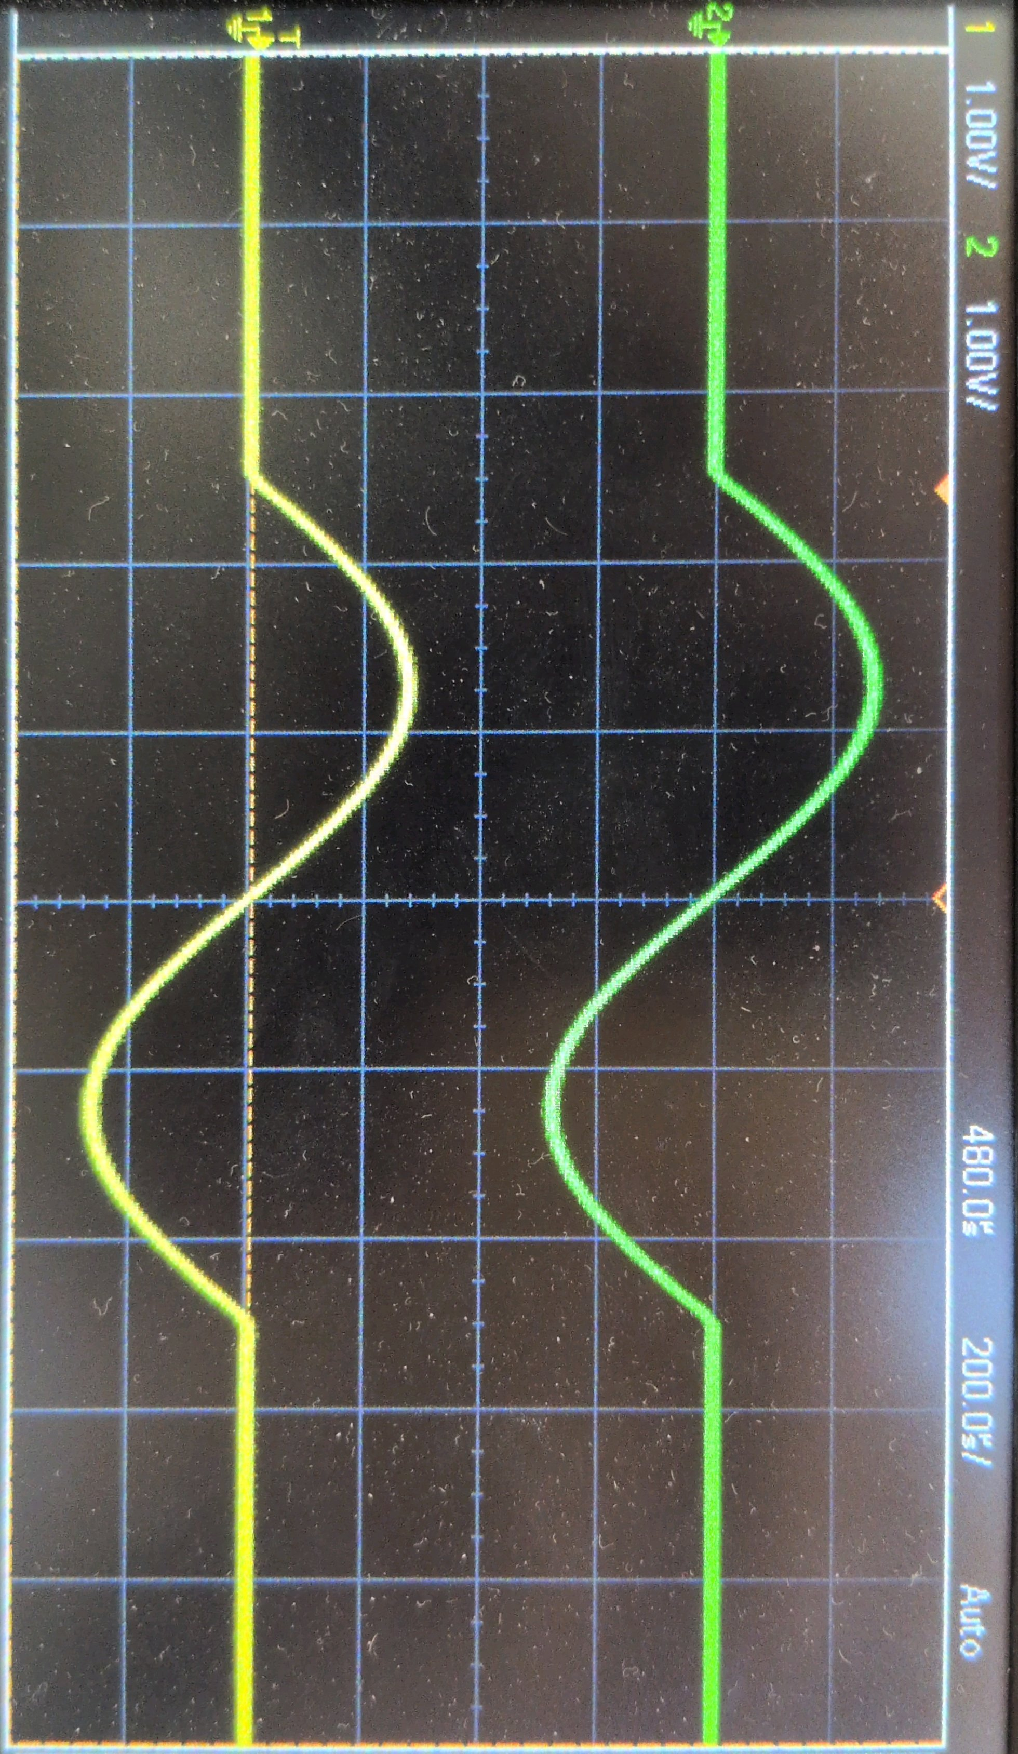
\includegraphics[height=\textwidth, angle=90]{osciloskop/6_kontrola_faze.pdf}
    \caption{Kontrola fáze.}
\end{figure}

\section{Použité přístroje}

\begin{itemize}
	\item \textbf{GEN} disky AVP \& Marutech CD generator a Sony Test CD type 3
	\item \textbf{DVD} přehrávač DVD Pioneer DV-585 (ve funkci CD-A přehrávače)
	\item \textbf{NZ} napájecí zdroj Diametral (napájení $\pm$12V, +5V)
	\item \textbf{OSC} paměťový osciloskop Agilent Technologies DSO3102A
	\item \textbf{ANA} audio analyzátor Rohde \& Schwarz UP350
	\item měřený přípravek „Digitální ekvalizer a limiter nf signálu“
	\item propojovací vodiče 4 x cinch--cinch, 4 x redukce BNC--cinch
\end{itemize}

\section{Závěr}

\end{document}